\documentclass[11pt]{article}
\usepackage{geometry}                
\geometry{letterpaper}                 
\usepackage[parfill]{parskip}        
\usepackage{graphicx}
\usepackage{amssymb}
\usepackage{amsmath}
\usepackage{epstopdf}
\usepackage{verbatim}
\usepackage{float}
\usepackage{enumerate}
\usepackage{hyperref}
\usepackage[utf8]{inputenc}
\usepackage[T1]{fontenc}
\DeclareGraphicsRule{.tif}{png}{.png}{`convert #1 `dirname #1`/`basename #1 .tif`.png}
\usepackage{color}
\usepackage{textcomp}
\definecolor{listinggray}{gray}{0.9}
\definecolor{lbcolor}{rgb}{1,1,1}

\begin{document}

\section*{Problems for Discussion 2, 09/18/13}
Compiled by Mai Le, some problems from Prof. Fessler and Prof. Yagle
% $x[n]$ can refer to a sequence or a value

\section{Discrete-domain Basis Sequences}
Let $x[n] = \{\underline{1},1,2,3,5\}$. Represent $x[n]$ in each of the following bases. 

Note: You won't be asked to do anything like this on the homework or exams, but hopefully it will help you solidify your understanding of bases from lecture.

\subsection*{Unit Step Sequences}
Recall $u[n] = \begin{cases}1, & n \geq 0\\ 0, & n < 0 \end{cases}$. Let $\mathcal{S}_u = \{u[n-n_0]|n_0 \in \mathbb{Z}\}$ (unit steps shifted by any integer $n_0$) be your basis sequences. Represent $x[n]$ in $\mathcal{S}_u$.

In other words, show you can write $x[n]=\sum\limits_{k=-\infty}^\infty c_k u[n-k]$ by finding the values for $c_k$.

{\color{blue}
$c = \{\underline{1}, 0, 1, 1, 2, -5\}$
}

\subsection*{Three-Tap Rectangles}
Let $r[n] = \{\underline{1},1,1\}$ and $\mathcal{S}_r = \{r[n-n_0]|n_0 \in \mathbb{Z}\}$. Represent $x[n]$ in $\mathcal{S}_r$.

{\color{blue}
$c = \{\underline{1}, 0, 1, 2, 0, 2, -4, 2, 2, -4, 2, 2, -4, \ldots \}$
}

\subsection*{Three-Tap Triangle}
Let $t[n] = \{\underline{1},2,1\}$ and $\mathcal{S}_t = \{t[n-n_0]|n_0 \in \mathbb{Z}\}$. Represent $x[n]$ in $\mathcal{S}_t$.

{\color{blue}
$c = \{\underline{1}, -1, 3, -2, 6, -10, 14, -18, \ldots \}$
}


\section{Properties of Even More Systems}
Are the following linear? time-invariant? causal? stable?


{\color{blue} 
Proofs omitted for brevity. If you have questions, post on Piazza or come to office hours!
}

\subsection*{(a)}

$y[n] = x^2[n+1]$

{\color{blue}
linear? no \\
time-invariant? yes \\
causal? no \\
stable? yes \\
}

\subsection*{(b)}

$y[n]=\begin{cases}x[-n], & n < 0\\ x[n], & n \geq 0 \end{cases} $

{\color{blue}
linear? yes \\
time-invariant? no \\
causal? no \\
stable? yes \\
}

\subsection*{(c)}

$y[n] = \sum_{k=-\infty}^{\infty}x[n-k]p[k]$ where $p[n] = \{-10,\ldots,-1,\underline{0},1,\ldots,10\}$.

{\color{blue}
linear? yes \\
time-invariant? yes \\
causal? no \\
stable? yes \\
}

%\section{Decomposition of Signals into Even and Odd} 

\section{Proof of Parseval's Theorem}
Prove that $\sum_{n=-\infty}^\infty|x[n]|^2 = \frac{1}{2 \pi} \int_{- \pi}^\pi |X(\omega)|^2 d\omega$.

{\color{blue}
\begin{eqnarray*}
\text{energy in time domain } E &=& \sum\limits_{n=-\infty}^\infty |x[n]|^2 \\
&=& \sum\limits_{n=-\infty}^\infty x[n]x^*[n] \\
&=& \sum\limits_{n=-\infty}^\infty x[n]\left(\frac{1}{2 \pi} \int_{-\pi}^\pi X(\omega)e^{j\omega n} d\omega \right)^* \\
&=& \frac{1}{2 \pi} \int_{-\pi}^\pi X^*(\omega) \left( \sum\limits_{n=-\infty}^\infty x[n]e^{-j\omega n}  \right)d\omega \\
&=& \frac{1}{2 \pi} \int_{-\pi}^\pi X^*(\omega) X(\omega) d\omega \\
&=& \frac{1}{2 \pi} \int_{-\pi}^\pi |X(\omega)|^2 d\omega  \text{ energy in the frequency domain}
\end{eqnarray*}

Thus, we see that energy is conserved by the DTFT (and IDTFT). (If you are curious about this, a more advanced interpretation of this result is that the DTFT is a unitary transformation!)
}

\section{Orthogonality of Complex Exponentials}

\subsection*{(a)}
Prove $\frac{1}{N}\sum\limits_{n=0}^{N-1} e^{j\frac{2 \pi}{N} k n} = \begin{cases}1, & k =0, \pm N, \pm 2N,... \\0, & otherwise \end{cases}$.

{\color{blue}
This solution will be withheld for now.
}

\subsection*{(b)} 
Show that harmonically related complex exponential signals $s_k[n]=e^{j\frac{2 \pi}{N} kn}$ are orthogonal over any interval of length $N$. I.e. $\sum\limits_{n=n_0}^{n_0+N-1} s_k[n]s_l^*[n] = 0$ if $k \neq l$.

{\color{blue}
This solution will be withheld for now.
}

\section{Symmetry and the DTFT}
\subsection*{(a)}

Let $y[n] = x^*[-n]$. What is $Y(\omega)$ in terms of $X(\omega)$?
{\color{blue}
\begin{eqnarray*}
Y(\omega) &=& \sum\limits_{n=-\infty}^\infty y[n]e^{-j\omega n} \\
&=& \sum\limits_{n=-\infty}^\infty x^*[-n]e^{-j\omega n} \\
&& \text{Let $m = -n$} \\
&=& \sum\limits_{m=\infty}^{-\infty} x^*[m]e^{j\omega m} = \sum\limits_{m=-\infty}^{\infty} x^*[m]e^{j\omega m} \\
&=& \sum\limits_{m=-\infty}^{\infty} \left( x^[m]e^{-j\omega m}\right)^* \\
&=& \left( \sum\limits_{m=-\infty}^{\infty}  x^[m]e^{-j\omega m}\right)^* \\
&=& X^*(\omega)
\end{eqnarray*}
}


\subsection*{(b)}

If $x[n]$ is real, what can we say about the symmetry of $X(\omega)$?

{\color{blue}
If $x[n]$ is real, then $x[n] = x^*[n]$. This is like part (a) without the time reversal. 

If we simply had $y[n] = x^*[n]$, then we could derive $Y(\omega) = X^*(-\omega)$ from steps similar to those in part (a). Since $x[n] = x^*[n] = y[n]$, then $X(\omega) = Y(\omega) = X^*(-\omega)$. This property is called "Hermitian symmetry", or "conjugate symmetry".
}

\section{Inverse DTFT}
\subsection*{(a) Inverse DTFT of a Triangle}
Find the signal $x[n]$ that has the following spectrum. Hint: integration by parts!

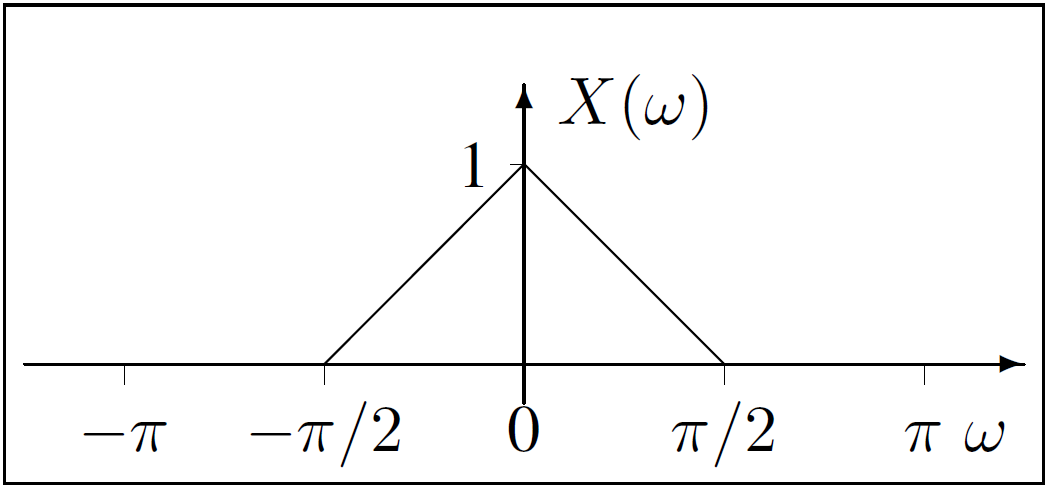
\includegraphics[scale=0.25]{fessler_hmwk6_p1.png}

{\color{blue}

There are multiple methods to solve this problem.

\subsubsection*{Method 1: Evaluating the integral directly}

First, we construct an expression for $X(\omega)$ as a function of $\omega$. $X(\omega) = \left(1-\big|\frac{2 \omega}{\pi}\big|\right)rect\left(\frac{\omega}{\pi}\right)$ Or equivalently, $X(\omega) = \left(1-\big|\frac{2 \omega}{\pi}\big|\right)\left(u\left(\omega+\frac{\pi}{2}\right)-u\left(\omega-\frac{\pi}{2}\right)\right)$.

Secondly, we need to recall the definition of the standard sinc function: $sinc(x) = \frac{sin(\pi x)}{\pi x}$. (This was covered in EECS 216, but it will be occasionally useful here in EECS 451.)

\begin{eqnarray*}
x[n] &=& \frac{1}{2 \pi} \int_{-\pi}^\pi X(\omega)e^{j\omega n}d\omega \text{ from the def'n of the IDTFT} \\
&=& \frac{1}{2 \pi} \int_{-\pi}^\pi \left(1-\big|\frac{2 \omega}{\pi}\big|\right)rect\left(\frac{\omega}{\pi}\right) e^{j\omega n}d\omega \\
&=& \frac{1}{2 \pi} \int_{-\frac{\pi}{2}}^{\frac{\pi}{2}} \left(1-\big|\frac{2 \omega}{\pi}\big|\right)e^{j\omega n}d\omega \\
%&=& \text{ BLACK MAGIC, INT BY PARTS} \\	
&=& \frac{2}{\pi^2 n^2} \left(1-cos\left(\frac{\pi}{2}n\right)\right) \\
\text{ using the trig identity: } && sin^2(\theta) = \frac{1}{2}\left( 1-cos(2\theta) \right) \\
&=& \frac{4 sin^2\left(\frac{\pi}{4}n\right)}{\pi^2 n^2} = \frac{1}{4}sinc^2\left(\frac{n}{4}\right) 
\end{eqnarray*}

\subsubsection*{Method 2: Using the Modulation Theorem}
We haven't covered it in lecture yet, but this method uses Eqn 7 of Table 2.2 (Fourier Transform Theorems) on page 59 of the 2nd edition (p. 58 in the 3rd edition). Essentially this theorem says that convolution in the frequency domain is equivalent to multiplication in the time domain.

So we seek to decompose $X(\omega)$ as a convolution of two other spectra: $X(\omega) = X_1(\omega)*X_2(\omega)$. $x[n]$ will then be the product of $x_1[n]$ and $x_2[n]$.
%
%Form inspection (and an intuition of convolution), we can show that:\\
%$X(\omega) = \left[\sqrt{\frac{2}{\pi}}rect\left(\frac{2}{\pi}\omega \right)\right] * \left[\sqrt{\frac{2}{\pi}}rect\left(\frac{2}{\pi}\omega \right)\right]$\\
%i.e. $X_1(\omega) = X_2(\omega) = \sqrt{\frac{2}{\pi}}rect\left(\frac{2}{\pi}\omega \right)$.
%
%Using the Fourier Transform Pair table, we see that the $IDTFT\left(rect(\frac{\omega}{2\omega_c}) \right) = \frac{sin(\omega_c n)}{\pi n} = \frac{\omega_c}{\pi^2} sinc(\frac{\omega_c}{\pi} n)$. 
%
%So we can find $x_1[n]=x_2[n]=\sqrt{\frac{2}{\pi}}\frac{sin\left(\frac{\pi}{4}n\right)}{\pi n}$. Should this be scaled by 4?
%
%
%Since $X(\omega)=X_1(\omega)*X_2(\omega)$, $x[n]=x_1[n]x_2[n] = \frac{2 sin^2\left( \frac{\pi}{4} n \right) }{\pi^3 n^2} = \frac{1}{4}sinc^2\left(\frac{n}{4}\right) $
%WHY DO I HAVE A CUBED TERM IN THE BOTTOM

The solution for this method will be posted at a later date.
}

\subsection*{(b)}
Given: $h[n] = \delta[n-1]+\delta[n+1]$ has spectrum $H(\omega) = 1 e^{-j\omega}+1e^{j\omega}=2cos(\omega)$. (You should be able to verify this.)

Find the signal $y[n]$ that has the spectrum $Y(\omega)=cos^2(\omega)$. (Don't do the integration!)

{\color{blue}
There are many ways to do this problem without evaluating the integral directly.

%\subsubsection*{Method 1: Using the time-shifting property of the DTFT}

\subsubsection*{Method 1: Using the convolution theorem} 

We can factor $Y(\omega) = Y_1(\omega)Y_2(\omega)$, where $Y_1(\omega) = Y_2(\omega) = cos(\omega)$.

What is the IDTFT of $cos(\omega)$? 
\begin{eqnarray*}
cos(\omega) &=& \frac{1}{2}\left(e^{j\omega}+e^{-j\omega}) \right) \\
IDTFT(cos(\omega)) &=& \frac{1}{2}\left(IDTFT(e^{j\omega})+IDTFT(e^{-j\omega})) \right) \\
y_1[n] = y_2[n] &=& \frac{1}{2}\left(\delta[n+1]+\delta[n-1] \right) \\
\end{eqnarray*}

From the convolution theorem, we know then that $y[n] = y_1[n]*y_2[n] = \frac{1}{2}\left(\delta[n+1]+\delta[n-1] \right) * \frac{1}{2}\left(\delta[n+1]+\delta[n-1] \right) = \frac{1}{4}\delta[n-2] + \frac{1}{2}\delta[n] + \frac{1}{4}\delta[n+2] $.


\subsubsection*{Method 2: Using trig identities and upsampling}

First, we consider what happens if you upsample $h[n]$. Let $h_2[n] = \delta[n-2]+\delta[n+2]$ has spectrum $H(\omega) = e^{-2j\omega}+e^{2j\omega}=2cos(2\omega)$. (You should also be able to verify this.)

Using trig identities, we can rewrite $Y(\omega) = cos^2(\omega) = \frac{1}{2} +\frac{1}{2}cos(2\omega)$. Using linearity of the IDTFT, we can invert each term separately. 
From the Fourier Transform pair table, we see that $IDTFT(1) = \delta[n]$, so $IDTFT\left(\frac{1}{2} \right) = \frac{1}{2}\delta[n]$. 
And from our previous analysis of $h_2[n]$, we can say that $IDTFT\left(\frac{1}{2}cos(2\omega)\right) = \frac{1}{4}\left(\delta[n-2]+\delta[n+2] \right)$. 
Thus, $y[n] = \frac{1}{2}\delta[n] + \frac{1}{4}\left(\delta[n-2]+\delta[n+2] \right)$.

}

\section{Inverse DTFT}
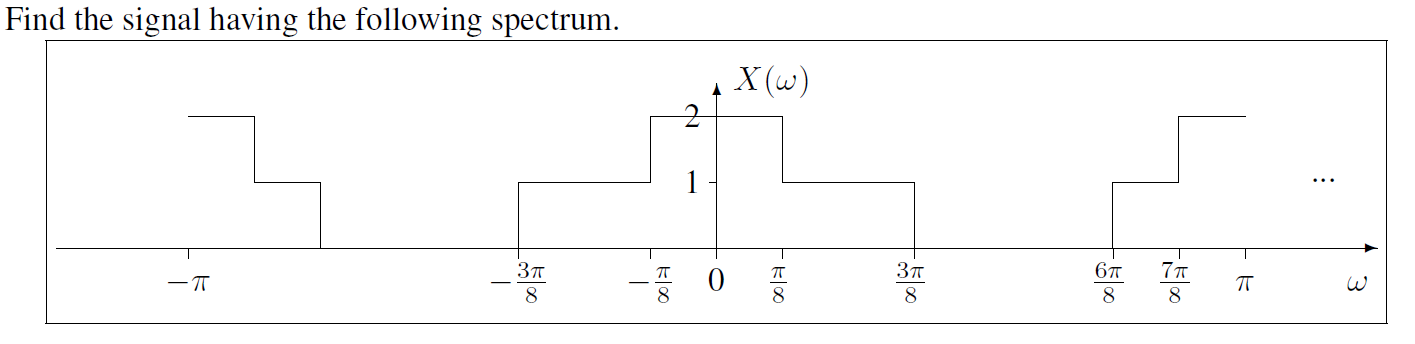
\includegraphics[width = \textwidth]{fessler_hmwk5_p9.png}

{\color{blue}
First, we seek to write an expression for $X(\omega)$. Though you could write $X(\omega)$ as a piecewise function, it is more useful to decompose $X(\omega)$ into the sum of simpler functions, such as rects. In this solution, I choose to break $X(\omega)$ down into four $rect$ functions, but you could decompose this in alternate ways.

$X(\omega) = A(\omega)+B(\omega)+C(\omega)+D(\omega)$ where $A(\omega), B(\omega), C(\omega), D(\omega)$ are as follows:

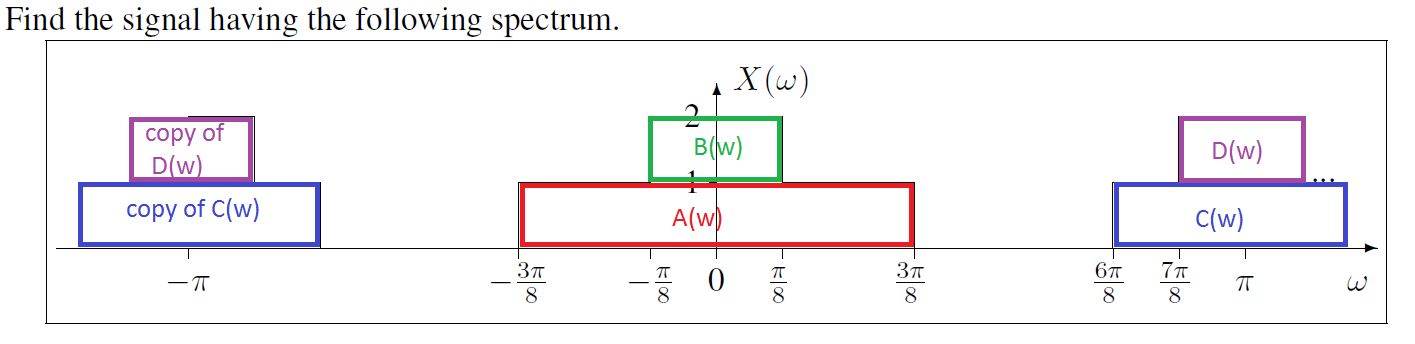
\includegraphics[width = \textwidth]{fessler_hmwk5_p9_annotated.png}

\begin{eqnarray*}
A(\omega) &=& rect\left( \frac{\omega}{\frac{3 \pi} {4} } \right)\\
B(\omega) &=& rect\left( \frac{\omega}{\frac{\pi} {4} } \right)\\
C(\omega) &=& rect\left( \frac{\omega - \pi}{\frac{\pi} {2} } \right)\\
D(\omega) &=& rect\left( \frac{\omega - \pi}{\frac{\pi} {4} } \right)
\end{eqnarray*}

Now we use the known DTFT pair:
$\frac{sin(\omega_c n)}{\pi n} \xrightarrow{\mbox{\tiny{DTFT}}}  rect\left(\frac{\omega}{2 \omega_c} \right)$

and the Frequency-Shifting Theorem (line 3 in Table 2.2):
$X(\omega-\omega_0) \xrightarrow{\mbox{\tiny{IDTFT}}} e^{j\omega_0 n} x[n]$.

\begin{eqnarray*}
IDTFT(A(\omega)) = a[n] &=& \frac{sin\left(\frac{3 \pi}{8}n\right)}{\pi n}\\
IDTFT(B(\omega)) = b[n] &=& \frac{sin\left(\frac{\pi}{8}n\right)}{\pi n}\\
IDTFT(C(\omega)) = c[n] &=& \frac{sin\left(\frac{\pi}{4}n\right)}{\pi n}e^{j \pi n} =\frac{sin\left(\frac{\pi}{4}n\right)}{\pi n}(-1)^{n}\\
IDTFT(D(\omega)) = d[n] &=& \frac{sin\left(\frac{\pi}{8}n\right)}{\pi n}e^{j \pi n} = \frac{sin\left(\frac{\pi}{8}n\right)}{\pi n}(-1)^{n}
\end{eqnarray*}

From the linearity of the IDTFT, 

$x[n] = a[n]+b[n]+c[n]+d[n] = (1 + (-1)^n)  \frac{sin\left(\frac{\pi}{8}n\right)}{\pi n} + \frac{sin\left(\frac{3 \pi}{8}n\right)}{\pi n} + \frac{sin\left(\frac{\pi}{4}n\right)}{\pi n}(-1)^{n}$. 

}

\end{document}